\section{Background}

%Describe the greater context, what are the technologies and protocols figuring in this thesis.
%In beginning mention a little bit of both IoT and ICN sort of waving them together.
%
%\begin{itemize}
%\item Describe the greater contest, what are the technologies and protocols figuring in the thesis.
%\item Mention both IoT and ICN and wave them together somehow.
%\item describe the growing number of IoT devices.
%\end{itemize}


A total of 26 billion IoT units installed world wide is estimated in the year of 2020. It represents a stagering 30 time increase from the year of 2009, where a total of 0.9 billion units was installed \cite{Gartner}. The increase in demand has led to that several major manufactures has joined the market, which in turn has led to several different communcation standards that the IoT devices communicates with. 

A new communication protocol are not developed overnight. It takes severe amount of reasearch and time to develope a new protocol. A majority of the network protocols and systems in this thesis were developed during the 1990s or early 2000. Although ICN was coined in 2000 with the TRIAD paper \cite{TRIAD}, it was not until 2009 when Jacobsson et al \cite{Jacobson2009} when it started to draw attention.

Each operating system and protocol of communication has its own restriction and possibility in delivering sensor data from a producer to a consumer.
In this section, systems and protcols used in this thesis is described that can be applied in wireless sensor networks.

\subsection{Internet of Things - network stack}

\begin{itemize}
	\item Write about growing number of devices
	\item how the devices come into play and where they're used.
	\item Describe the devices similarity, that they often are the same. High level of hetrogenous.
\end{itemize}


Write about the growing nubmer if devices. How they're coming into play and where they're used.

\subsubsection{IEEE 802.15.4}
The IEEE 802.15.4 standard intends to offer the fundamental lower network layers for wireless personal area networks (WPAN).  The standard focus is on providing a low cost, low power consumption and low data rates between inexpensive wireless devices. 
The standard only provides the MAC and PHY layers, leaving the upper layers to be chosen by the applicant\cite{6185525} \cite{radio-electronic-802-15-4}. Due to the special PHY layer and to keep the transmission times short and resistant against failures, it does not exchange standard Ethernet frames with maximum transmission unit (MTU) of 1500 octets. The MTU of 802.15.4 is instead set to 127 octets. The communication range is set up to 10 meter and a maximum data transfer rate limited at 250kbit/s. Depending on wireless technology and how constrained the device is, the maximum transmission speed can be set to as low as 20 kbit/s.
[<rewrite this>]
It is important to stress that the 802.15.4 standard does not compete with the regular 802.11 standard, where costs are not as critical and security and speed are more demanded. Today transfer rates up to gigabites is possible with the latest 802.11 standard, these speeds are hardly unneccesary in the IoT domain.[<\/rewrite this>]
\\\\
There are two different types of network nodes that can exist in a 802.15.4 network\cite{radio-electronic-802-15-4}. Full functional device(FFD) and reduced function device(RFD). A FFD node implements all communication funcionallity the 802.15.4 standard offer, it can communicate with any other device in the network. A FFD node may therefore also route data from other nodes. When doing that the node is also called a cooardinator. If all communication in the network is routed through a dedicated FFD node, it is called a PAN coardinatior. A RFD has a reduced level of functionallity and is meant to be extremly simple. Such devices are always an end node in a network and can only communicate through or with a FFD. They can never act as a cooardinator due to their limited capabilities.
\\\\
The two main network topology forms that are used within the 802.15.4 standard, are the star topology and the peer-to-peer topogoly, shown in figure \ref{fig:topology}. In star topology, all devices are required to only communicate to a single central device called the PAN controller. An advantage with this topology is that it makes it easy to manage and support. The drawbacks of using a star topology structure are bigger, for instance will it limit the area that can be covered geographically since all data has to be routed through one device and the distance a node can cover is set to be at a maximum of ten meters.\\
The peer-to-peer topology can have an arbitrary number of connections to each other within the network. Devices can communicate with each other, not only through the PAN controller, with exception for communication between RFDs. There are several advantages by using the peer-to-peer structure, for instance since devices can route traffic via other FFD devices, the network coverage can be easily increased.\\

%picture of the stuff.

\begin{figure}
	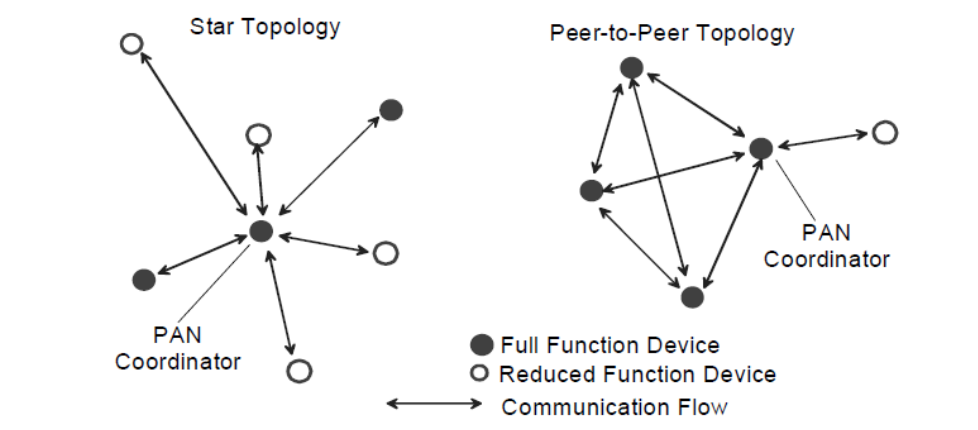
\includegraphics[width=\textwidth]{figures/802-15-4-topologies.png}
	%\caption{Star topology structure on the left, Peer-to-peer on the right. write where it is taken from?}
	\caption{Topology structures in 802.15.4 networks. Star structure on the left, Peer-to-peer on the right.}
	\label{fig:topology}
\end{figure}


% describe the difference and the importance of their functionallites.


exisiting usage of 802.15.4... maybe a subsection of Zigbee too?\\

\subsubsection{IPv4, IPv6}
Since the introduction of Internet Protocol version 4 (IPv4) in 1981\cite{rfc791}, it has been the backbone of the Internet and as the network layer in the OSI model. The protocol defines an address space of 32 bits and the total number of unique addresses that is available with IPv4 is around 4 billion. Today, the IPv4 address space is exhausting at a rapid speed and there is not enough addresses left to handle the increased number of devices that will be connected to the Internet in the future[Make citation!!].
\\\\
In response to the shortage of address space, among other things, the Internet Protocol version 6 (IPv6) was formulised and defined as a successor to IPv4 in 1998\cite{rfc2460}. The IPv6 protocol defines the length of an address of 128 bits, which lead to a total address space of ${2^{128}}$ equal to ${3.4*10^{38}}$ unique addresses. With an address space of this size, it will be sufficient for all IoT and Internet devices to have an own IP address. IPv6 requires that every link to the Internet has an MTU of 1280 octets or greater. In case this need can not be met,  fragmentation and reassembly must be provided at layer below IPv6\cite{rfc2460}.


% Maybee add some more about IPv6?

\subsubsection{6LowPAN}

At first glance, it may seem straightforward to send IPv6 data packets on a 802.15.4 network. However, there are incompabilities between the two formats making it hard for them to cooperate. For instance, the largest frame size of 802.15.4 (127 octets) is considerably less than the required MTU of IPv6 (1280 octets) \cite{rfc4944}. Futhermore, the IPv6 header is 40 octets long which is almost a third of the total 802.15.4 MTU (at least 25 octets). This leaves only 62 octets for upper-layer protocols as UDP or ICMP. That makes it impossible in the first case and infeasable in the second, to build IPv6 direclty on top of the 802.15.4 MAC layer as in a regular IP protocol on the Ethernet MAC layer in the IP stack, shown in figure \ref{fig:ip-6lowpan-stack}.\\\\
To address these issues, among several, ``IPv6 over Low-Power Wireless Personal Area Networks'' (6LoWPAN) was established in 2007 as an adoption layer between the IEEE 802.15.4 MAC-layer and IPv6. 6LowPAN makes it possible to transfer IPv6 packets over a 802.15.4 network through fragmentation and reassembly, and IPv6- and UDP header compressions to shrink the packet size. Through header compression strategies, it is possible to shrink down the IPv6- and UDP header, toward as little as 4 octets in total (instead of 48 octets) \cite{rfc4944}. Other features of 6LowPAN is the neighbor discovery and mesh routing support. Even though there is no limitation to only use UDP, for simplicity and performance reasons it is more favorable to use UDP over TCP as the transport protocol with 6LowPAN.


\begin{figure}
	%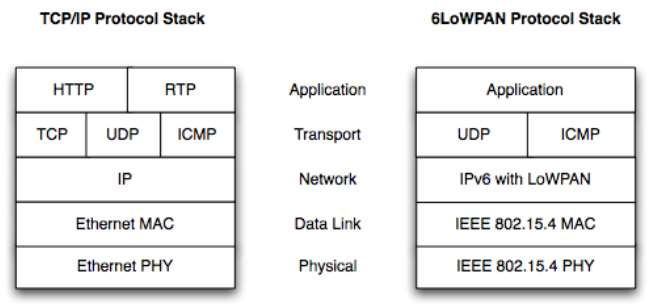
\includegraphics[width=\textwidth]{figures/ip-6lowpan-stack.jpg}
	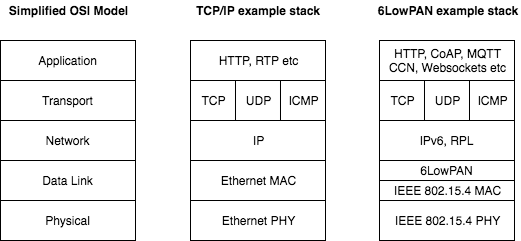
\includegraphics[width=\textwidth]{figures/6lowpan-own.png}
	%\caption{Star topology structure on the left, Peer-to-peer on the right. write where it is taken from?}
	%\caption{Simplified OSI model, an example TCP/IP stack and an illustration of the 6LowPAN protocol stacks, copied from \cite{rfc4944}}
	\caption{The simplified OSI model, an example TCP/IP stack and an illustration of an example 6LowPAN protocol stacks.}
	\label{fig:ip-6lowpan-stack}
\end{figure}

\subsubsection{MQTT, MQTT-SN}
Message Queuing Telemetry Transport(MQTT) is a open lightweight publish-subscribe messageing protocol, designed for constrained devices with low-bandwidth and/or unreliable networks targeting Machine-to-Machine (M2M) communication\cite{mqtt}. The protocol reside in the application layer in the OSI model, assuming that the underlaying network structure provides a point-to-point, session-oriented data transport provided by example TCP/IP \cite{hunkeler2008mqtt}. This assumption makes the protocol unsuitable for devices that can not hold their own TCP/IP stack, which lead to MQTT-SN described further down. The publish-subscribe message pattern require a message broker, which is responsible for distributing messages to the interested clients.
\\\\
The publish-subscribe pattern can be described by a server, or sensor, acting as a publisher/producer of information and a client as the consumer/subscriber of information. A client subscribes on a specific topic, set of data, that resides on the server/sensor. When the server has produced data for the specific topic, it will send that information towards the client. 
The information is going through a broker that handles all the information regarding which devices subscribe to which publisher. The broker is usually located in a traditional network due to its higher performance regarding bandwith and processing capabilities.\\\\
MQTT-SN, where the extension stands for sensor network, is a MQTT version that is adapted for wireless communication. It is optimized to be implemented on low-cost, battery-operated devices with limited or constrained storage and processing capabilities\cite{MQTT-SN}, perticular targeting IoT and sensor devices.\\
Where MQTT uses string characters as topic names, MQTT-SN uses numeric IDs which reduce the size of the packets in favor of readability. Furthermore, MQTT-SN, in contrast to MQTT, does not depend on a connection-oriented transport service (TCP/IP), it is able to work with other transport protocols such as UDP/IP, ZigBee or others. 

[more about brokers and its role.]

\subsubsection{CoAP}
The Constrained Application Protocol (CoAP) is a specialized web transfer protocol to be used with constrained devices and networks, and between M2M communication\cite{rfc7959}. CoAP resides in the application layer, above transport layer, in the OSI model stack.
It provides a client/server interaction model between application endpoints similar to the HTTP standard. 
CoAP is based on the REST architecture and follows the general design to manipulate data in a request/response manner. The methods GET, POST, PUT and DELETE are similar to HTTP, but not identical.
\\\\
While HTTP uses TCP as transportation protocol, CoAP data is sent asynchronously over a datagram-oriented protocol such as UDP. Due to the implementation of UDP, features like resend lost datapackets, and acknowledge-messages are missing in the transport layer[ref kid]. This functionallity has in some extent been moved into the CoAP protocol and is called Messages. \\
CoAP defines four different type of messages: confirmable, non-confirmable, acknowledgment, reset. They occupy 2 bit out of 32 bit of the total CoAP header.
A confirmable message provides reliability by retransmitting a message until a recipient sends an Acknowledgment message with the same Message ID back to the requester. If a requested message can not be handled by the recipient, a reset message will replied instead. When a message does not require reliable transmission (no acknowledgment is needed), a non-confirmable message is sent. These non-confirmable messages will still have a message ID in order to detect duplication.

[note, maybe reorder so first coap, then request/response, then Messages? Add about in network caching? Also add source to second paragraph]















\subsection{Information Centric Networking}
Information-Centric Networking (ICN) is a communication paradigm for the future Internet that is based on \textit{named data} instead of \textit{named hosts}. It represents an evolution of the Internet from todays host-centric networking, in particular IP networking, towards an information-centric approach.

There are several different approaches of implementing the ICN paradigm, but there are fundamental ideas that they all follow regardless which implementation is used. This section will continue describing the general ideas. However, the thesis overall will only consider the \textit{Content Centric networking} approach described more in depth at the next section.

Some of the main features in the ICN are the possibility of in-network storage for caching data, multiparty communication through replication, decoupling senders and receivers, and that data is named\cite{Ahlgren2012}. In information-centric networks, an information request may not only be satisfied by locating the original information source, it is possible for any of the in-network caches to reply to the request with the desired data if they hold any copies of it. After a request is sent from a user, it is the responsibility of the network to locate the best source that can provide the information. Due to the fact that information/data is named, addressed and matched independently from its location, the data may be located anywhere in the network[icn research][18][19]. Hence the argument that the ICN approach decouple the information from its source.




\subsubsection{Content-Centric Networking}



%\begin{itemize}
%\item motivation, one type of ICN architecture. 
%\end{itemize}
The CCN communication \cite{Jacobson2009} is driven by consumers of data. There are two types of message in CCN, \textit{Interest} and \textit{Data}. A consumer issues an \textit{Interest} message to request an information object on the network. Any node that recieved the interest and containing the requested information, will respond by sending the \textit{Data} back to the \textit{Interest} issuer. A \textit{Data} message is only sent in response to an \textit{Interest} message, upon response, the interest message will cease to exist in the network. This implies that the data that a producer creates will only reach the network, or any participant of the network, if there is a request for it.

A key feature of CCN is that the content names are hierarchical. This allows routing information to be aggregated which in turn is critical in order to scale the network. The content name can be simila to URLs, for example a valid content name could be \textit{/sics.se/kista/floor/six/sensor/two/temperature}. However, there is neither a strict need for them to be human-readable nor tobe a URL. The prefix \textit{/sics.se/kista/floor/six/sensor/two/} could easily be exchanged to become either a hash value or just an integer, say \textit{2} (representing the sensor two), whereby the same data could be accessable by the name \textit{/2/temperature}.

It is to be considered an interest match  when any part of the interest name equals the named prefix of the data, for example is it possible that \textit{/2/temperature} could be match by \textit{/2/temperature/sequence$\_$1}. If the data is produced periodically with sequence numbering, a consumer can `follow' the data by the same manner once it has a starting point. %\todo{Explain what is meant by hit/b}

Even though there are a lot of similiarities to regular routers IP, there are a lot of differences between a CCN router and a regular IP router.
Every Content Router (CR) maintain three main data structures: The Forwarding Information Base (FIB), the Pending Interest Table (PIT) and the Content Store (CS).

The FIB is used to map information to on which output interface a Interest message should be forwarded to in order to reach its content. It is very similar to a regular FIB in a IP router, with the major difference that the CCN FIB allows lists of outgoing interfaces instead if just a single entry per object.

The PIT maintain a table for all incoming \textit{interests} messages recieved by the CR, their current state and a mapping to which face they came from. When the data message for a particular \textit{interest} arrives to a CR, the data message will be forwarded back on a reverse path, towards the face that exist in the corresponding PIT entry. After the data message has been forwarded towards the requester, its entry in the PIT will be erased. Whenever an entry is dropped or lost, for instance due to timeouts, it is up to the consumer to issue a new \textit{interest} message.\

The CS act as a local cache for information objects that has passed through the CR.

With the use of the CRs, CCN has great support for data caching. As stated earlier, once a \textit{interest} is receievd, the CR will look through its CS in order to find matching data. Once the data is on the reverse path to the consumer, it will be put in the CS for a limited period of time for futhre use. Although there are several benefits using the cache in a distributed network system, it should be pointed out that this is not a long-term storage since a router can not hold infinite number of data. Nor is it useful for data objects that are requested at most once, since the benefits only occur when the data is requested a second time \cite{Ahlgreniot}\cite{Ahlgren2012}. %[Ahlgren2][surveyiot].
\\\\
An example of CCN in action is illustraded in figure \ref{fig:CCN-architecture}. Here, a consumer wants to retrive the indoor temperature data from the producer.
Consumer1 sends an \textit{interest} for data \textit{/temp/indoor} towards CR1. When it arrives, CR1 looks for data in its CS that matches the requested prefix of the interest. Since there is no match in the CS, the router performs a lookup on the longest prefix that matches its FIB in order to decide where to forward the incoming interest. When the match in the FIB is found, the router inserts the interest, with the incoming interface, into the PIT.

The same procedure happens for CR2 and the interest will be put in the PIT and forwarded to the producer. When the \textit{interest} reaches the producer, it matches the name of the \textit{data} and thereby the \textit{interest} message is discarded and the \textit{data} is sent back towards CR2. When the data is received, CR2 stores the data in the cache. Thereafter it performs a longest-prefix match in its PIT to get which interface it should respond to. In this case, it will respond to CR1 and the same forward back procedure will occur at CR1 until the data reaches the consumer.

When Consumer2 later on wants the same content, it sends an \textit{interest} to CR1 and will retreive the data directly from its cache and thereby reducing the network traffic.



\begin{figure}
	%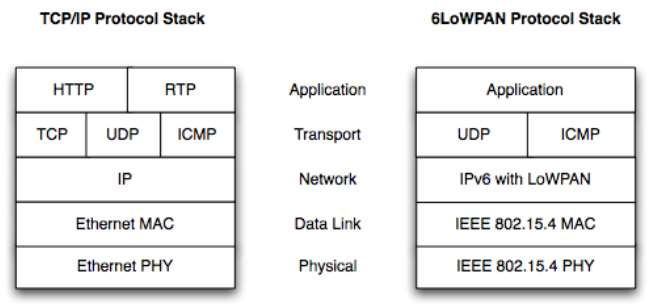
\includegraphics[width=\textwidth]{figures/ip-6lowpan-stack.jpg}
	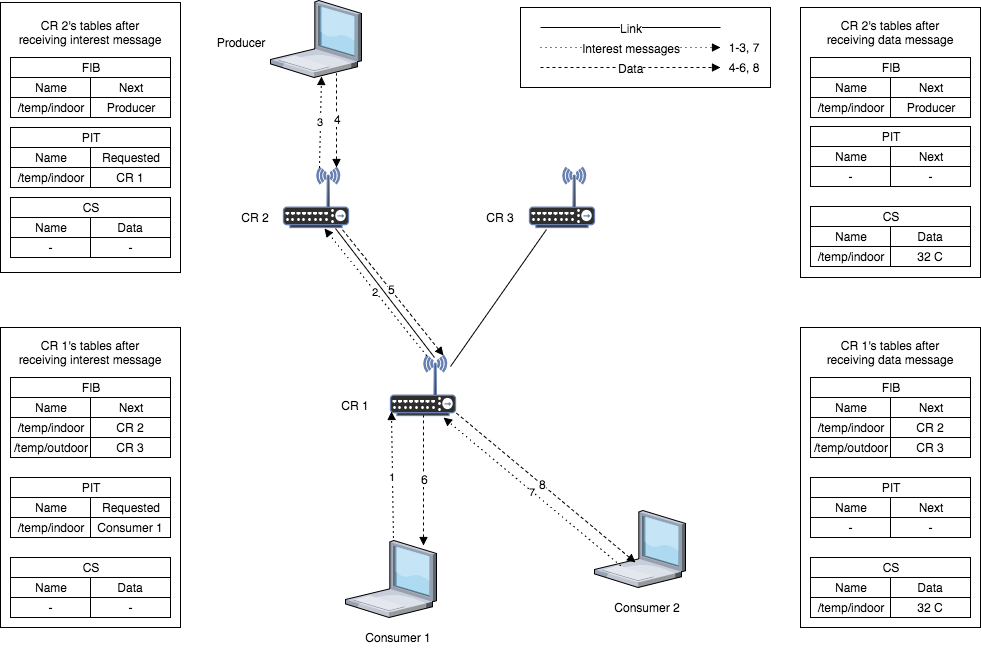
\includegraphics[width=\textwidth]{figures/CCN-architecture.png}
	%\caption{Star topology structure on the left, Peer-to-peer on the right. write where it is taken from?}
	%\caption{Simplified OSI model, an example TCP/IP stack and an illustration of the 6LowPAN protocol stacks, copied from \cite{rfc4944}}
	\caption{The CCN architecture builed up by content routers (CR), forwarding information base (FIB), pending interest table (PIT) and content store (CS), inspired by [ref survey ICN]}
	\label{fig:CCN-architecture}
\end{figure}



\subsubsection{Using ICN for IoT}
The usage of IoT devices most often implies an information centric pattern. In many scenarios, the main goal is the data and services and it is less important to communicate with a specific device \cite{Ahlgreniot}. Where users and/or devices rather consume content, generated by an IoT device, through the network than connecting directly to a specific device or host. Therefore one could argue that naming the data is more important than naming the devices.

Depending on topology structure of the IoT network, the caching mechanisms ICN provides could help constrained IoT devices to avoid unnecessary transmissions when distributing its data into multiple places. Storing cached data in the network could also potentially save energy and network bandwidth of an IoT device.

% There are several reasons why it is better to use an ICN approach in the IoT domain. Everything always depends on application and usage, but there are some pros and cons using ICN in the IoT domain.
% 
% \begin{itemize}
% 	\item + naming of data
% 	\item + distributed caching
% 	\item + Decoupling between publisher and consumer
% 	\item + Sending request for the future.
% 	\item advantages of using ICN in IoT domain.
% 	\item disadvantages
% 	Even though the major advantage of using named data in IoT, it comes with some concerns. How to create and format efficient names suitable for huge numbers.
% \end{itemize}




\subsubsection{CCN-lite}
CCN-lite is a lightweight, functionally implementation of CCN \cite{CCN-LITE}. There are several platforms that are supported such as UNIX, Linux, Android, Arduino and several other. It uses a small code base of C, less than 2000 lines of code, in order to implement the CCN functionality. CCN-lite runs over UDP and Ethernet, and support packet fragmentation.
\\






















\subsection{Contiki-OS}
Contiki OS is an open source operating system that is suitable for network-connected, memory-constrained devices that targeting Internet of Things \cite{contiki-os}. It focus on wireless technologies and implement a number of IoT protocols including 6LoWPAN, IEEE 802.15.4, RPL, CoAP and MQTT. Contiki provides a full IP network stack with protocols as IPv4, IPv6, TCP, UDP and HTTP. It is designed to operate with extreme low-power systems.

%\subsubsection{6LBR}
%In order to connect a device to the Internet one can use the 6LowPAN Border Router, 6LBR\cite{6LBR}. It is implemented on Contiki-OS and provide interconnection between IP and 6LowPAN networks. The router assumes an Ethernet interface on the IP side and 802.15.4 on the sensor side. Devices connected to the 802.15.4-to-Ethernet gateway can reach and be reachable to/from the Internet. There is no native support for IPv4, altough there are mechanisms to achive some IPv4 funcitonallity through a NAT64. [is this contributing any to the thesis? Or should it be more focus on Sparrow.]

\subsubsection{Sparrow}
Sparrow is a commnunication format that encapsulates different types of payload on top of IPv6/UDP \cite{Sparrow}. The Sparrow border router is based on the original Contiki border router but it has been improved with additional features. It acts as the RPL root and handles all the routing towards the sensors and maintains the network as a whole. The software makes it possible to initiate and hold communications with the remote sensortags. The border router connects the sensor network to the local host (Linux/OS-X or other), making it possible for the applications on the host to reach nodes in the sensor network. 

\subsubsection{CCN-lite portation}
%Yanqui Wu, former thesis worker at SICS, implemented and ported a version of the CCN-lite \cite{CCN-LITE} to the Contiki-OS platform in 2016 \cite{yanqui}. The software is to be considered laying in the application layer and will not replace any other layers in the OSI model. It handles all necessary functionallity that the regular CCN-lite application provides. Depending on how much memory that is available at the hardware, one can tune in how many entries that the PIT-table and the content store can hold. 
Yanqui Wu, former thesis worker at SICS, implemented and ported a version of the CCN-lite \cite{CCN-LITE} to the Contiki-OS platform in 2016 \cite{yanqui}. The portation enables a sensor to send and receive its application data with the ICN communication pattern providing a subset of the functionallity that the regular CCN-lite provides. A consumer can send an \textit{interest} message to the sensor, running with Contiki software, in order to receieve the \textit{data}. Depending on how much memory available at the sensor, one one can tune in how many entries that the PIT-table and the content store can contain.



%\subsection{Hardware}

\subsubsection{Texas Instrument CC2650 SensorTag}
The CC2650 sensortag is a wireless microcontroller developed by Texas Instruments \cite{CC2650}. The device is low cost, ultralow power device using the 2.4 Ghz radiofrequency to communicate with technologies such as 6LowPAN, Bluetooth and Zigbee. Due to its ultra low power consumption, the sensor can be powered by battery.
The CC2650 device contains a 32-bit ARM Cortex-M3 processor running at 48 Mhz, accompanied by 8 KB of cache and 20 KB of SRAM. It contains a total of 128 KB of programable flash memory, which can be used for different application system such as the Contiki-OS system. The sensor controller supports the measurement of different types of sensor data such as temperature readings, optical light values and more. 


\subsubsection{Zolertia Firefly Slip radio}
The Firefly radio slip is developed by Zolertia \cite{Firefly}. The radio slip provides a network infrastructure for the IoT devices, enabling them to communicate efficiently through the air. The Firefly has great routing capabilities due to its support for several communication technologies, among them IEEE 802.15.4/6LowPAN and Zigbee. Another advantage using the Firefly is that it supports multiple types of frequency bands such as 2.4 GHz, 915- and 920 MHz band. Radio parameters such as modulation, data rate and transmission power are highly configurable.

\subsubsection{Raspberry Pi 3}
The Raspberry Pi 3 is a single board computer developed by the Raspberry Pi Foundation \cite{RP3}. It contains components suchs as WIFI, several USB ports, 1 GB RAM and a quad core ARM processor among several other features. Due to its relativly high performance for a low price, it has become a popular developing tool used in projects at home, in school and for academic research.
